% Options for packages loaded elsewhere
\PassOptionsToPackage{unicode}{hyperref}
\PassOptionsToPackage{hyphens}{url}
%
\documentclass[
  10pt,
  a4paper,
]{article}
\usepackage{amsmath,amssymb}
\usepackage{iftex}
\ifPDFTeX
  \usepackage[T1]{fontenc}
  \usepackage[utf8]{inputenc}
  \usepackage{textcomp} % provide euro and other symbols
\else % if luatex or xetex
  \usepackage{unicode-math} % this also loads fontspec
  \defaultfontfeatures{Scale=MatchLowercase}
  \defaultfontfeatures[\rmfamily]{Ligatures=TeX,Scale=1}
\fi
\usepackage{lmodern}
\ifPDFTeX\else
  % xetex/luatex font selection
\fi
% Use upquote if available, for straight quotes in verbatim environments
\IfFileExists{upquote.sty}{\usepackage{upquote}}{}
\IfFileExists{microtype.sty}{% use microtype if available
  \usepackage[]{microtype}
  \UseMicrotypeSet[protrusion]{basicmath} % disable protrusion for tt fonts
}{}
\makeatletter
\@ifundefined{KOMAClassName}{% if non-KOMA class
  \IfFileExists{parskip.sty}{%
    \usepackage{parskip}
  }{% else
    \setlength{\parindent}{0pt}
    \setlength{\parskip}{6pt plus 2pt minus 1pt}}
}{% if KOMA class
  \KOMAoptions{parskip=half}}
\makeatother
\usepackage{xcolor}
\usepackage[margin=20mm]{geometry}
\usepackage{longtable,booktabs,array}
\usepackage{calc} % for calculating minipage widths
% Correct order of tables after \paragraph or \subparagraph
\usepackage{etoolbox}
\makeatletter
\patchcmd\longtable{\par}{\if@noskipsec\mbox{}\fi\par}{}{}
\makeatother
% Allow footnotes in longtable head/foot
\IfFileExists{footnotehyper.sty}{\usepackage{footnotehyper}}{\usepackage{footnote}}
\makesavenoteenv{longtable}
\usepackage{graphicx}
\makeatletter
\def\maxwidth{\ifdim\Gin@nat@width>\linewidth\linewidth\else\Gin@nat@width\fi}
\def\maxheight{\ifdim\Gin@nat@height>\textheight\textheight\else\Gin@nat@height\fi}
\makeatother
% Scale images if necessary, so that they will not overflow the page
% margins by default, and it is still possible to overwrite the defaults
% using explicit options in \includegraphics[width, height, ...]{}
\setkeys{Gin}{width=\maxwidth,height=\maxheight,keepaspectratio}
% Set default figure placement to htbp
\makeatletter
\def\fps@figure{htbp}
\makeatother
\setlength{\emergencystretch}{3em} % prevent overfull lines
\providecommand{\tightlist}{%
  \setlength{\itemsep}{0pt}\setlength{\parskip}{0pt}}
\setcounter{secnumdepth}{-\maxdimen} % remove section numbering
\usepackage{float}
\usepackage{fancyhdr}
\pagestyle{fancy}\fancyhf{}
\fancyhead[L]{\small FMAT3888: Portfolio Construction}
\fancyhead[R]{\small Question 4(a)--(c)}
\fancyfoot[C]{\thepage}
\setlength{\headheight}{14pt}
\setlength{\parskip}{4pt}
\usepackage{needspace}
\ifLuaTeX
  \usepackage{selnolig}  % disable illegal ligatures
\fi
\IfFileExists{bookmark.sty}{\usepackage{bookmark}}{\usepackage{hyperref}}
\IfFileExists{xurl.sty}{\usepackage{xurl}}{} % add URL line breaks if available
\urlstyle{same}
\hypersetup{
  hidelinks,
  pdfcreator={LaTeX via pandoc}}

\author{}
\date{}

\begin{document}

\hypertarget{question-4-utility-monte-carlo-and-portfolio-uncertainty}{%
\section{Question 4: Utility, Monte Carlo and Portfolio
Uncertainty}\label{question-4-utility-monte-carlo-and-portfolio-uncertainty}}

Priority 1 - Essential: Include to answer Q4(a)-(c), justify the model
and explain the conclusions.

Priority 2 - Supporting evidence: Include if space permits; otherwise
summarise or move to an appendix.

Priority 3 - Optional detail: Keep in the repository or appendix unless
additional space is available.

\begin{longtable}[]{@{}
  >{\raggedright\arraybackslash}p{(\columnwidth - 2\tabcolsep) * \real{0.4286}}
  >{\raggedleft\arraybackslash}p{(\columnwidth - 2\tabcolsep) * \real{0.5714}}@{}}
\toprule\noalign{}
\begin{minipage}[b]{\linewidth}\raggedright
Report item
\end{minipage} & \begin{minipage}[b]{\linewidth}\raggedleft
Priority
\end{minipage} \\
\midrule\noalign{}
\endhead
\bottomrule\noalign{}
\endlastfoot
Return horizon, Q1 inputs, constraints and utility objective & 1 \\
Full derivation of the normal-model utility formula & 2 \\
Risk-aversion values and their justification & 1 \\
Optimal allocations, expected returns, volatility and interpretation &
1 \\
Figure 1: risk-aversion outcomes and allocation heatmap & 2 \\
Monte Carlo methods, sample sizes and accuracy measures & 1 \\
Stable numerical objective and gradient details & 2 \\
Monte Carlo accuracy, runtime and benchmark comparison & 1 \\
Figure 2 and detailed gamma-by-gamma Monte Carlo comparison & 2 \\
Historical bootstrap design and re-estimation procedure & 1 \\
Bootstrap allocation uncertainty and interpretation & 1 \\
Figure 3: bootstrap uncertainty visualisation & 2 \\
Moving-block bootstrap experiment & 3 \\
Bootstrap replication-count check & 2 \\
Main conclusion and modelling limitations & 1 \\
Detailed numerical checks, coverage checklist and handover & 3 \\
\end{longtable}

\newpage

\hypertarget{model-and-modelling-choices-priority-1}{%
\subsection{Model and modelling choices {[}Priority
1{]}}\label{model-and-modelling-choices-priority-1}}

Question 4 investigates how an investor's attitude toward risk affects
their optimal portfolio and how reliable that portfolio is. Part (a)
finds the optimal allocations for different levels of risk aversion.
Part (b) checks whether Monte Carlo simulation can reproduce those
solutions accurately and efficiently. Part (c) uses historical bootstrap
samples to examine how much the optimal weights change when estimated
returns and covariances change. Together, these parts help us understand
both which portfolio suits a given risk preference and how much
confidence we should place in its estimated weights. The portfolios are
fully invested, short selling is excluded, and each index has a 50\%
allocation limit.

\hypertarget{return-horizon-and-utility-priority-1}{%
\subsubsection{Return horizon and utility {[}Priority
1{]}}\label{return-horizon-and-utility-priority-1}}

We model returns over one year using a normal distribution,

\[
R\sim N(m,C)
\]

Using Q1's annualised estimates,

\[
m=12\times\text{average monthly return}
\]

\[
C=12\times\text{sample monthly covariance matrix}
\]

This arithmetic approximation does not account for compounding or
dependence between returns in different months.

\hypertarget{supporting-utility-derivation-priority-2}{%
\subsubsection{Supporting utility derivation {[}Priority
2{]}}\label{supporting-utility-derivation-priority-2}}

The investor has initial wealth \(W_0\) = 1, terminal wealth:

\[
W_1=1+x^\top R
\]

and exponential utility:

\[
U(W)=-\exp(-\gamma W)
\]

Under the normal return model:

\[
\mathbb E[U(W_1)]=-\exp\!\left[-\gamma(1+x^\top m)+\frac{\gamma^2}{2}x^\top Cx\right]
\]

Maximising expected utility is therefore equivalent to maximising:

\[
f_\gamma(x)=x^\top m-\frac{\gamma}{2}x^\top Cx
\]

The first term is expected portfolio return. The second is the variance
penalty, weighted by risk aversion.

The certainty-equivalent return is the guaranteed return an investor
would consider equally attractive to the risky portfolio. Under our
model: \[
f_\gamma(x)=\text{expected return}-\frac{\gamma}{2}\times\text{variance}
\]

For example, if \(f_\gamma(x)\) = 0.05, the investor considers the risky
portfolio equally attractive to a guaranteed 5\% return. Since initial
wealth is 1, certainty-equivalent final wealth is 1 + \(f_\gamma(x)\) .

A larger \(\gamma\) gives a larger risk penalty, lowering the certainty
equivalent of the same portfolio. Utility comparisons between portfolios
should use the same \(\gamma\) because changing \(\gamma\) changes the
investor's preferences.

\hypertarget{choosing-the-risk-aversion-range-priority-1}{%
\subsubsection{Choosing the risk-aversion range {[}Priority
1{]}}\label{choosing-the-risk-aversion-range-priority-1}}

We use \(\gamma\) = 1, 5, 10, 25 and 100 to represent different levels
of risk aversion. These values were selected after testing a wider range
and show how allocations shift from higher-return assets toward
lower-risk assets as risk aversion increases. They illustrate different
investor preferences rather than identify a single best \(\gamma\).

\hypertarget{q4a-optimal-portfolios-under-different-risk-aversion-priority-1}{%
\subsection{Q4(a): Optimal portfolios under different risk aversion
{[}Priority
1{]}}\label{q4a-optimal-portfolios-under-different-risk-aversion-priority-1}}

As C is positive definite and \(\gamma\) \textgreater{} 0, the objective
is strictly concave. For each \(\gamma\), the model has a unique optimal
portfolio. We calculate its weights numerically and check that they
satisfy the full-investment, no-short-selling and 50\% cap constraints,
as well as the conditions for optimality.

\begin{longtable}[]{@{}
  >{\raggedright\arraybackslash}p{(\columnwidth - 6\tabcolsep) * \real{0.2000}}
  >{\raggedleft\arraybackslash}p{(\columnwidth - 6\tabcolsep) * \real{0.2667}}
  >{\raggedleft\arraybackslash}p{(\columnwidth - 6\tabcolsep) * \real{0.2667}}
  >{\raggedleft\arraybackslash}p{(\columnwidth - 6\tabcolsep) * \real{0.2667}}@{}}
\toprule\noalign{}
\begin{minipage}[b]{\linewidth}\raggedright
Risk aversion \(\gamma\)
\end{minipage} & \begin{minipage}[b]{\linewidth}\raggedleft
Expected annual return
\end{minipage} & \begin{minipage}[b]{\linewidth}\raggedleft
Annual volatility
\end{minipage} & \begin{minipage}[b]{\linewidth}\raggedleft
CE return
\end{minipage} \\
\midrule\noalign{}
\endhead
\bottomrule\noalign{}
\endlastfoot
1 & 9.551\% & 11.623\% & 8.876\% \\
5 & 8.510\% & 9.252\% & 6.371\% \\
10 & 6.611\% & 5.609\% & 5.038\% \\
25 & 4.732\% & 2.441\% & 3.987\% \\
100 & 3.982\% & 1.398\% & 3.004\% \\
\end{longtable}

\hypertarget{portfolio-allocations-priority-1}{%
\subsubsection{Portfolio allocations {[}Priority
1{]}}\label{portfolio-allocations-priority-1}}

\begin{longtable}[]{@{}
  >{\raggedright\arraybackslash}p{(\columnwidth - 10\tabcolsep) * \real{0.1304}}
  >{\raggedleft\arraybackslash}p{(\columnwidth - 10\tabcolsep) * \real{0.1739}}
  >{\raggedleft\arraybackslash}p{(\columnwidth - 10\tabcolsep) * \real{0.1739}}
  >{\raggedleft\arraybackslash}p{(\columnwidth - 10\tabcolsep) * \real{0.1739}}
  >{\raggedleft\arraybackslash}p{(\columnwidth - 10\tabcolsep) * \real{0.1739}}
  >{\raggedleft\arraybackslash}p{(\columnwidth - 10\tabcolsep) * \real{0.1739}}@{}}
\toprule\noalign{}
\begin{minipage}[b]{\linewidth}\raggedright
Index
\end{minipage} & \begin{minipage}[b]{\linewidth}\raggedleft
\(\gamma\) = 1
\end{minipage} & \begin{minipage}[b]{\linewidth}\raggedleft
\(\gamma\) = 5
\end{minipage} & \begin{minipage}[b]{\linewidth}\raggedleft
\(\gamma\) = 10
\end{minipage} & \begin{minipage}[b]{\linewidth}\raggedleft
\(\gamma\) = 25
\end{minipage} & \begin{minipage}[b]{\linewidth}\raggedleft
\(\gamma\) = 100
\end{minipage} \\
\midrule\noalign{}
\endhead
\bottomrule\noalign{}
\endlastfoot
ASA52 & 0.00\% & 0.00\% & 0.00\% & 0.00\% & 0.00\% \\
NDDLWI & 25.22\% & 12.24\% & 0.00\% & 0.00\% & 0.00\% \\
NDLEEGF & 24.78\% & 18.20\% & 8.43\% & 2.20\% & 0.00\% \\
RDAU & 0.00\% & 0.00\% & 0.00\% & 0.00\% & 0.00\% \\
FDCIISAH & 50.00\% & 50.00\% & 33.35\% & 12.00\% & 0.00\% \\
HEDGNAV & 0.00\% & 0.00\% & 15.64\% & 15.02\% & 19.48\% \\
BACM0 & 0.00\% & 0.00\% & 17.65\% & 9.63\% & 11.39\% \\
H03432AU & 0.00\% & 19.56\% & 24.92\% & 16.40\% & 19.13\% \\
BAUBIL & 0.00\% & 0.00\% & 0.00\% & 44.75\% & 50.00\% \\
\end{longtable}

\textbf{Figure 1 - Priority 2}

\begin{figure}[H]
\centering
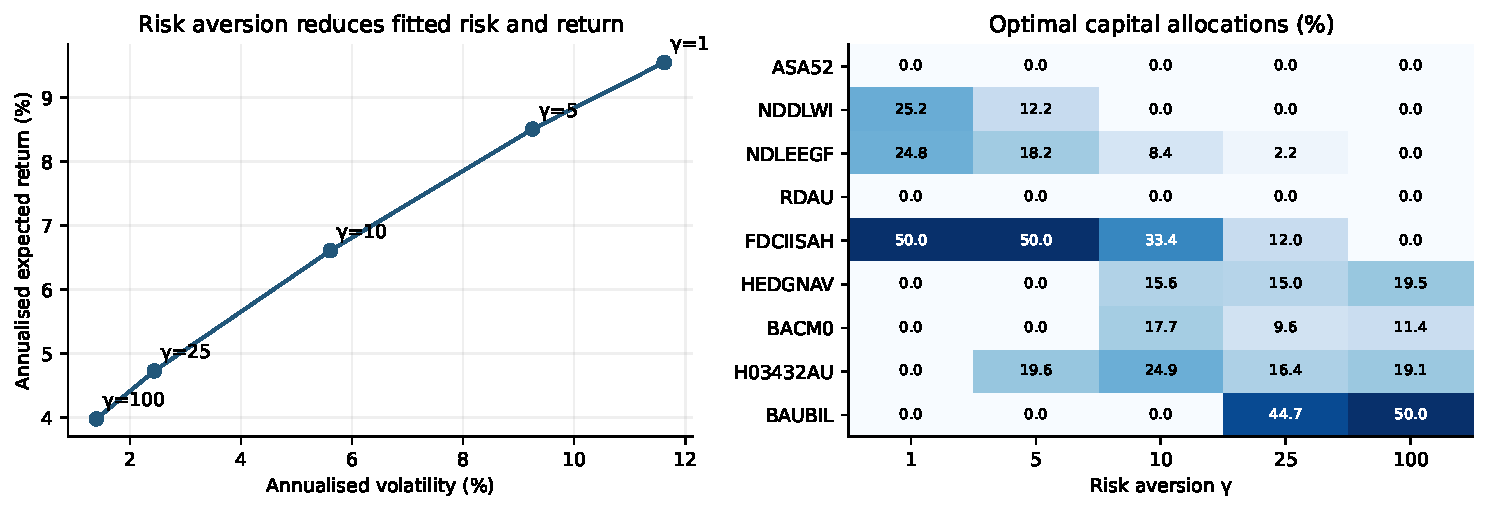
\includegraphics{../figures/Q4a_risk_aversion.pdf}
\caption{Fitted risk-return choices and capital allocations under
increasing risk aversion. All scenarios use the same historical
estimates and constraints.}
\end{figure}

\hypertarget{interpretation-priority-1}{%
\subsubsection{Interpretation {[}Priority
1{]}}\label{interpretation-priority-1}}

At \(\gamma\) = 1, the optimal portfolio combines NDDLWI, NDLEEGF and a
50\% holding in FDCIISAH. As risk aversion rises, lower-risk assets
enter and both fitted return and volatility fall.

At \(\gamma\) = 25, BAUBIL receives approximately 44.75\%. At \(\gamma\)
= 100, it reaches its 50\% cap. The latter portfolio's volatility,
1.398\%, is close to capped GMV's 1.383\%. However, utility optimisation
still rewards expected return and therefore does not produce exactly the
GMV weights.

The outcome follows the trade-off in \(f_\gamma\) where a larger
\(\gamma\) places more weight on variance. These portfolios are optimal
conditional on the model, estimated inputs and preference value. They
are not universally optimal investment recommendations.

\hypertarget{q4b-numerical-expected-utility-optimisation-priority-1}{%
\subsection{Q4(b): Numerical expected-utility optimisation {[}Priority
1{]}}\label{q4b-numerical-expected-utility-optimisation-priority-1}}

\hypertarget{monte-carlo-implementation-priority-1}{%
\subsubsection{Monte Carlo implementation {[}Priority
1{]}}\label{monte-carlo-implementation-priority-1}}

For each experiment, we generate one-year arithmetic return vectors
using the Cholesky factor L of C:

\[
R^{(k)}=m+LZ^{(k)},\qquad Z^{(k)}\sim N(0,I)
\]

where m represents estimated expected returns, \(Z^{(k)}\) represents
independent random normal shocks, and L, calculated from C, transforms
those shocks so the simulated assets have the required risks and
correlations.

The Monte Carlo simulated expected utility is therefore: \[
\widehat{\mathbb E[U(W_1)]}=-e^{-\gamma}\frac1N\sum_{k=1}^{N}e^{-\gamma x^\top R^{(k)}}
\]

We then determine the portfolio weights that maximise this simulated
average utility, subject to the same portfolio constraints as Q4(a).

\hypertarget{stable-numerical-objective-priority-2}{%
\subsubsection{Stable numerical objective {[}Priority
2{]}}\label{stable-numerical-objective-priority-2}}

Maximising expected utility is equivalent to minimising the following
objective:

\[
h_N(x)=\frac1\gamma\log\!\left[\frac1N\sum_{k=1}^{N}e^{-\gamma x^\top R^{(k)}}\right]
\]

We evaluate this using log-sum-exp for numerical stability. Its gradient
is the negative return mean under exponential weights.

This solves the sampled expected-utility problem directly. It does not
replace that problem with a sample mean-variance approximation.

\hypertarget{simulation-procedure-priority-1}{%
\subsubsection{Simulation procedure {[}Priority
1{]}}\label{simulation-procedure-priority-1}}

Return draws remain fixed throughout each optimisation, making the
objective smooth and reproducible. Each run starts from equal weights
rather than the exact benchmark.

We also compare standard Monte Carlo with the toolbox's antithetic
method, using paired shocks to reduce simulation variance:

\[
m+LZ\qquad\text{and}\qquad m-LZ
\]

N counts the total number of return vectors. Therefore, antithetic Monte
Carlo uses N/2 independent pairs.

Samples are shared across the five preference scenarios within an
experiment and are not redrawn at every solver evaluation.

\hypertarget{experimental-choices-and-accuracy-measures-priority-1}{%
\subsubsection{Experimental choices and accuracy measures {[}Priority
1{]}}\label{experimental-choices-and-accuracy-measures-priority-1}}

We test:

\[
N=1{,}000,\ 10{,}000,\ 100{,}000
\]

Each method and sample size uses eight independent replications. This
tenfold ladder tests the accuracy-cost trade-off rather than selecting
one unexplained simulation count.

The fixed seed is 388804. Separate child streams are used for Monte
Carlo, ordinary bootstrap and block bootstrap.

Allocation distance measures how differently capital is allocated
compared with the benchmark. It was calculated using:

\[
D(x,\hat x)=\frac12\sum_i|x_i-\hat x_i|
\]

This is the fraction of capital allocated differently. It is not
realised trading turnover.

We also evaluate each Monte Carlo portfolio under the exact original
normal model, using the certainty-equivalent loss, which measures the
reduction in CE return from using the Monte Carlo allocation instead of
the benchmark:

\[
\text{CE loss}=f_\gamma(x^*)-f_\gamma(\hat x)\ge0
\]

Here, \(x^*\) is the exact benchmark allocation and \(\hat x\) is the
Monte Carlo allocation.

This avoids judging a simulated portfolio only by its optimised
in-sample utility. One basis point of CE return equals 0.0001.

The exported results also report CE estimation error and relative
expected-utility error at the fixed exact benchmark.

\hypertarget{numerical-accuracy-and-computational-performance-priority-1}{%
\subsubsection{Numerical accuracy and computational performance
{[}Priority
1{]}}\label{numerical-accuracy-and-computational-performance-priority-1}}

The following summaries give each risk-aversion scenario equal
representation. Allocation distance and CE loss are means over the five
scenarios and eight replications. Timing is the median across those
runs.

\begin{longtable}[]{@{}
  >{\raggedright\arraybackslash}p{(\columnwidth - 8\tabcolsep) * \real{0.1579}}
  >{\raggedleft\arraybackslash}p{(\columnwidth - 8\tabcolsep) * \real{0.2105}}
  >{\raggedleft\arraybackslash}p{(\columnwidth - 8\tabcolsep) * \real{0.2105}}
  >{\raggedleft\arraybackslash}p{(\columnwidth - 8\tabcolsep) * \real{0.2105}}
  >{\raggedleft\arraybackslash}p{(\columnwidth - 8\tabcolsep) * \real{0.2105}}@{}}
\toprule\noalign{}
\begin{minipage}[b]{\linewidth}\raggedright
Method
\end{minipage} & \begin{minipage}[b]{\linewidth}\raggedleft
N
\end{minipage} & \begin{minipage}[b]{\linewidth}\raggedleft
Mean allocation distance
\end{minipage} & \begin{minipage}[b]{\linewidth}\raggedleft
Mean CE loss (bp)
\end{minipage} & \begin{minipage}[b]{\linewidth}\raggedleft
Median time (ms)
\end{minipage} \\
\midrule\noalign{}
\endhead
\bottomrule\noalign{}
\endlastfoot
Antithetic & 1,000 & 7.97\% & 1.157 & 3.00 \\
Antithetic & 10,000 & 2.65\% & 0.087 & 5.74 \\
Antithetic & 100,000 & 0.56\% & 0.008 & 35.03 \\
Standard & 1,000 & 12.25\% & 1.758 & 2.65 \\
Standard & 10,000 & 4.10\% & 0.202 & 5.85 \\
Standard & 100,000 & 1.67\% & 0.044 & 37.99 \\
\end{longtable}

\textbf{Figure 2 - Priority 2}

\begin{figure}[H]
\centering
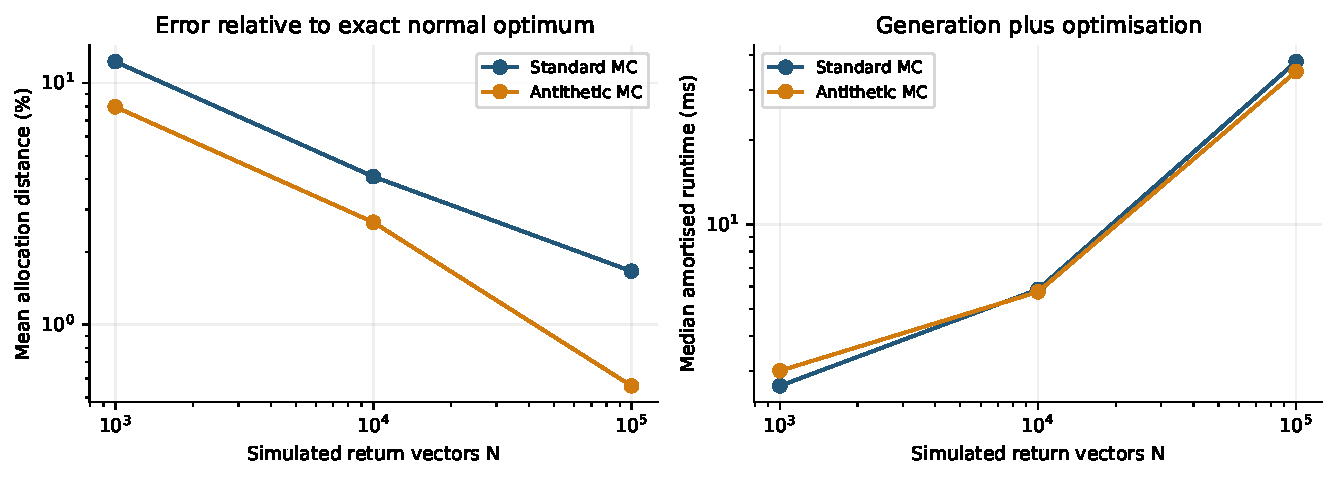
\includegraphics{../figures/Q4b_accuracy_runtime.pdf}
\caption{Allocation error and runtime as the number of simulated return
vectors increases. Runtime includes optimisation plus an equal share of
the one-time generation cost reused across preference scenarios.}
\end{figure}

The results show that:

\begin{itemize}
\tightlist
\item
  Larger samples reduced aggregate allocation error and CE loss.
\item
  Antithetic sampling improved aggregate accuracy in this experiment.
\end{itemize}

At N = 100,000, mean allocation distance is 1.67\% for standard Monte
Carlo and 0.56\% for antithetic Monte Carlo. Mean exact-model CE loss is
0.044 bp and 0.008 bp, respectively.

\needspace{10\baselineskip}

\hypertarget{detailed-comparison-by-risk-aversion-priority-2}{%
\subsubsection{Detailed comparison by risk aversion {[}Priority
2{]}}\label{detailed-comparison-by-risk-aversion-priority-2}}

The scenario-level comparison at N = 100,000 is:

\begin{longtable}[]{@{}
  >{\raggedright\arraybackslash}p{(\columnwidth - 8\tabcolsep) * \real{0.1579}}
  >{\raggedleft\arraybackslash}p{(\columnwidth - 8\tabcolsep) * \real{0.2105}}
  >{\raggedleft\arraybackslash}p{(\columnwidth - 8\tabcolsep) * \real{0.2105}}
  >{\raggedleft\arraybackslash}p{(\columnwidth - 8\tabcolsep) * \real{0.2105}}
  >{\raggedleft\arraybackslash}p{(\columnwidth - 8\tabcolsep) * \real{0.2105}}@{}}
\toprule\noalign{}
\begin{minipage}[b]{\linewidth}\raggedright
Risk aversion \(\gamma\)
\end{minipage} & \begin{minipage}[b]{\linewidth}\raggedleft
Standard distance
\end{minipage} & \begin{minipage}[b]{\linewidth}\raggedleft
Antithetic distance
\end{minipage} & \begin{minipage}[b]{\linewidth}\raggedleft
Standard CE loss (bp)
\end{minipage} & \begin{minipage}[b]{\linewidth}\raggedleft
Antithetic CE loss (bp)
\end{minipage} \\
\midrule\noalign{}
\endhead
\bottomrule\noalign{}
\endlastfoot
1 & 3.01\% & 0.37\% & 0.0799 & 0.0012 \\
5 & 1.78\% & 0.53\% & 0.0630 & 0.0137 \\
10 & 2.15\% & 0.95\% & 0.0511 & 0.0133 \\
25 & 1.10\% & 0.68\% & 0.0215 & 0.0071 \\
100 & 0.29\% & 0.27\% & 0.0037 & 0.0038 \\
\end{longtable}

\hypertarget{interpretation-and-benchmark-comparison-priority-1}{%
\subsubsection{Interpretation and benchmark comparison {[}Priority
1{]}}\label{interpretation-and-benchmark-comparison-priority-1}}

Allocation error and economic objective error need not move together:
nearby portfolios can have almost the same utility. Consequently, both
metrics are needed.

In this experiment, N = 100,000 provides the most accurate tested
aggregate approximation, at higher computational cost (longer time
taken). Eight replications give a limited assessment of simulation
variability, not a universal accuracy guarantee.

The exact quadratic benchmark takes approximately 0.80-1.33 ms per
solve. Antithetic Monte Carlo at N = 100,000 takes approximately 23-39
times longer for the solver alone.

Timings use one BLAS thread, exclude file input/output, and are
machine-specific. Benchmark timing is the median of 30 solves per
scenario. Monte Carlo timings include reoptimisation from equal weights.

Ultimately, for this normal/exponential-utility problem, the
mean-variance benchmark is preferable because it uses the exact
mean-variance reduction for the stated model, solved numerically under
the constraints, and is computationally less costly. Monte Carlo
provides a numerical validation here and becomes useful when an
analytical reduction is unavailable.

\hypertarget{q4c-historical-sampling-uncertainty-priority-1}{%
\subsection{Q4(c): Historical sampling uncertainty {[}Priority
1{]}}\label{q4c-historical-sampling-uncertainty-priority-1}}

\hypertarget{resampling-design-priority-1}{%
\subsubsection{Resampling design {[}Priority
1{]}}\label{resampling-design-priority-1}}

We create each bootstrap sample by randomly selecting 248 historical
months with replacement. All nine returns from a sampled month stay
together, preserving their relationship within that month. For each
sample, we re-estimate both the monthly mean and covariance, applying
Q1's annualisation of mean and covariance, and optimise the portfolio
again for every \(\gamma\) value.

We do not resample assets independently or hold the covariance matrix
fixed.

We use 10,000 independent and identically distributed (IID) resamples,
following a smaller pilot in which some tail endpoints changed
substantially.

At this count, the Monte Carlo standard error of an estimated selection
probability is at most 0.5 percentage points, and each 2.5\% tail
contains approximately 250 observations. Weight percentiles can
nevertheless remain unstable when many allocations are exactly zero or
at the 50\% cap. We therefore compare 5,000 with 10,000 replications
separately below.

The 2.5\%-97.5\% marginal ranges describe the resampled allocation
distribution under the chosen resampling scheme. They are not
future-return predictions or a joint confidence region for the
portfolio. Combining their endpoints does not necessarily produce
weights that sum to 100\%.

\hypertarget{allocation-stability-across-preferences-priority-1}{%
\subsubsection{Allocation stability across preferences {[}Priority
1{]}}\label{allocation-stability-across-preferences-priority-1}}

\begin{longtable}[]{@{}
  >{\raggedright\arraybackslash}p{(\columnwidth - 6\tabcolsep) * \real{0.2000}}
  >{\raggedleft\arraybackslash}p{(\columnwidth - 6\tabcolsep) * \real{0.2667}}
  >{\raggedleft\arraybackslash}p{(\columnwidth - 6\tabcolsep) * \real{0.2667}}
  >{\raggedleft\arraybackslash}p{(\columnwidth - 6\tabcolsep) * \real{0.2667}}@{}}
\toprule\noalign{}
\begin{minipage}[b]{\linewidth}\raggedright
Risk aversion \(\gamma\)
\end{minipage} & \begin{minipage}[b]{\linewidth}\raggedleft
Median allocation distance
\end{minipage} & \begin{minipage}[b]{\linewidth}\raggedleft
95th percentile distance
\end{minipage} & \begin{minipage}[b]{\linewidth}\raggedleft
Largest weight SD (percentage points)
\end{minipage} \\
\midrule\noalign{}
\endhead
\bottomrule\noalign{}
\endlastfoot
1 & 40.15\% & 75.22\% & 23.96 \\
5 & 41.78\% & 81.80\% & 19.42 \\
10 & 48.30\% & 73.92\% & 19.82 \\
25 & 35.74\% & 63.03\% & 18.62 \\
100 & 10.14\% & 20.19\% & 9.77 \\
\end{longtable}

For \(\gamma\) = 10, median allocation distance is 48.30\%, meaning that
the median bootstrap portfolio allocates 48.30\% of capital differently
from the original portfolio, with a 95th percentile of 73.92\%.

At \(\gamma\) = 100, the median distance is much smaller, approximately
10.14\%, although significant uncertainty remains.

Higher risk aversion is not uniformly more stable. The intermediate
mixed portfolios are particularly sensitive to estimated means and
covariances.

Now examining the portfolio specifically for \(\gamma\) = 10, the
marginal allocation ranges are:

\begin{longtable}[]{@{}
  >{\raggedright\arraybackslash}p{(\columnwidth - 8\tabcolsep) * \real{0.1579}}
  >{\raggedleft\arraybackslash}p{(\columnwidth - 8\tabcolsep) * \real{0.2105}}
  >{\raggedleft\arraybackslash}p{(\columnwidth - 8\tabcolsep) * \real{0.2105}}
  >{\raggedleft\arraybackslash}p{(\columnwidth - 8\tabcolsep) * \real{0.2105}}
  >{\raggedleft\arraybackslash}p{(\columnwidth - 8\tabcolsep) * \real{0.2105}}@{}}
\toprule\noalign{}
\begin{minipage}[b]{\linewidth}\raggedright
Index
\end{minipage} & \begin{minipage}[b]{\linewidth}\raggedleft
Fitted weight
\end{minipage} & \begin{minipage}[b]{\linewidth}\raggedleft
Bootstrap mean
\end{minipage} & \begin{minipage}[b]{\linewidth}\raggedleft
2.5th percentile
\end{minipage} & \begin{minipage}[b]{\linewidth}\raggedleft
97.5th percentile
\end{minipage} \\
\midrule\noalign{}
\endhead
\bottomrule\noalign{}
\endlastfoot
ASA52 & 0.00\% & 3.77\% & 0.00\% & 33.22\% \\
NDDLWI & 0.00\% & 6.65\% & 0.00\% & 40.15\% \\
NDLEEGF & 8.43\% & 8.64\% & 0.00\% & 37.83\% \\
RDAU & 0.00\% & 0.26\% & 0.00\% & 2.31\% \\
FDCIISAH & 33.35\% & 25.35\% & 0.00\% & 50.00\% \\
HEDGNAV & 15.64\% & 12.88\% & 0.00\% & 50.00\% \\
BACM0 & 17.65\% & 16.64\% & 0.00\% & 50.00\% \\
H03432AU & 24.92\% & 18.14\% & 0.00\% & 50.00\% \\
BAUBIL & 0.00\% & 7.65\% & 0.00\% & 50.00\% \\
\end{longtable}

FDCIISAH's fitted weight is 33.35\%, while H03432AU's is 24.92\%. Both
have bootstrap ranges extending from zero to 50\%.

Similarly, an asset receiving zero weight in the original portfolio may
receive a positive allocation in other samples.

This distinction between a unique fitted optimum and an uncertain
estimated optimum is central to Q4(c).

\hypertarget{visual-uncertainty-priority-2}{%
\subsubsection{Visual uncertainty {[}Priority
2{]}}\label{visual-uncertainty-priority-2}}

\begin{figure}[H]
\centering
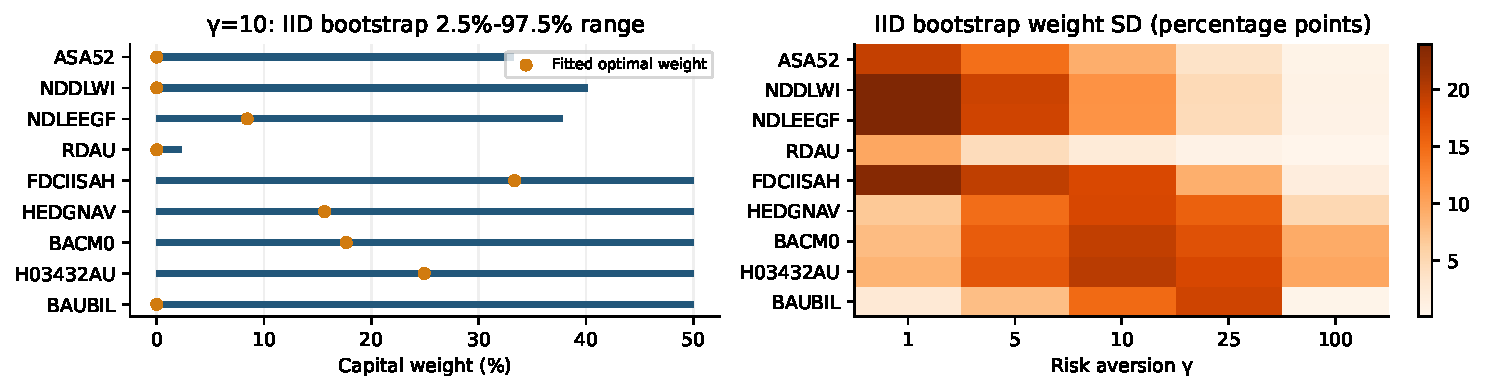
\includegraphics{../figures/Q4c_bootstrap_uncertainty.pdf}
\caption{IID bootstrap allocation ranges for \(\gamma\) = 10 and
marginal allocation standard deviations across the preference scenarios.
The dots show the original fitted allocation; the bands show resampling
variability.}
\end{figure}

\hypertarget{independence-limitation-priority-1}{%
\subsubsection{Independence limitation {[}Priority
1{]}}\label{independence-limitation-priority-1}}

The ordinary bootstrap treats months as independent. However, returns
may be related across consecutive months. The observed lag-one
correlations are approximately 0.982 for BAUBIL and 0.219 for HEDGNAV,
so this assumption is a limitation.

\hypertarget{moving-block-sensitivity-experiment-priority-3}{%
\subsubsection{Moving-block sensitivity experiment {[}Priority
3{]}}\label{moving-block-sensitivity-experiment-priority-3}}

As a sensitivity check, we resample joint moving blocks of 6, 12 and 24
months. We sample valid historical block starts uniformly, concatenate
the blocks, and truncate the resulting sample to 248 rows.

This preserves dependence within each block while retaining the same
estimation and optimisation conventions. Twelve months matches the
one-year stated model. Six and 24 months test shorter and longer
dependence retention. These are transparent sensitivity choices, not an
estimated optimal block length.

Each length uses 1,000 replications, so block results are coarser than
the primary IID experiment. This is an additional historical-bootstrap
sensitivity check, not a replacement of the assignment's normal return
model or Q1 covariance convention.

Median allocation distances are:

\begin{longtable}[]{@{}
  >{\raggedright\arraybackslash}p{(\columnwidth - 8\tabcolsep) * \real{0.1579}}
  >{\raggedleft\arraybackslash}p{(\columnwidth - 8\tabcolsep) * \real{0.2105}}
  >{\raggedleft\arraybackslash}p{(\columnwidth - 8\tabcolsep) * \real{0.2105}}
  >{\raggedleft\arraybackslash}p{(\columnwidth - 8\tabcolsep) * \real{0.2105}}
  >{\raggedleft\arraybackslash}p{(\columnwidth - 8\tabcolsep) * \real{0.2105}}@{}}
\toprule\noalign{}
\begin{minipage}[b]{\linewidth}\raggedright
Risk aversion \(\gamma\)
\end{minipage} & \begin{minipage}[b]{\linewidth}\raggedleft
IID months
\end{minipage} & \begin{minipage}[b]{\linewidth}\raggedleft
6-month blocks
\end{minipage} & \begin{minipage}[b]{\linewidth}\raggedleft
12-month blocks
\end{minipage} & \begin{minipage}[b]{\linewidth}\raggedleft
24-month blocks
\end{minipage} \\
\midrule\noalign{}
\endhead
\bottomrule\noalign{}
\endlastfoot
1 & 40.15\% & 29.16\% & 43.25\% & 27.19\% \\
5 & 41.78\% & 40.12\% & 43.59\% & 40.59\% \\
10 & 48.30\% & 47.66\% & 48.71\% & 47.62\% \\
25 & 35.74\% & 36.09\% & 40.23\% & 38.85\% \\
100 & 10.14\% & 10.05\% & 9.90\% & 9.40\% \\
\end{longtable}

The intermediate allocations remain highly uncertain under every
resampling scheme. For \(\gamma\) = 10, the 12-month-block median
distance is approximately 48.71\%, close to the IID value.

The schemes do not produce identical distributions, and block resampling
does not mechanically increase every uncertainty measure. Their
agreement on substantial instability is more useful than treating a
particular interval endpoint as exact.

\hypertarget{replication-count-check-priority-2}{%
\subsubsection{Replication-count check {[}Priority
2{]}}\label{replication-count-check-priority-2}}

Comparing the first 5,000 IID resamples with all 10,000 gives:

\begin{longtable}[]{@{}
  >{\raggedright\arraybackslash}p{(\columnwidth - 4\tabcolsep) * \real{0.2727}}
  >{\raggedleft\arraybackslash}p{(\columnwidth - 4\tabcolsep) * \real{0.3636}}
  >{\raggedleft\arraybackslash}p{(\columnwidth - 4\tabcolsep) * \real{0.3636}}@{}}
\toprule\noalign{}
\begin{minipage}[b]{\linewidth}\raggedright
Risk aversion \(\gamma\)
\end{minipage} & \begin{minipage}[b]{\linewidth}\raggedleft
Maximum mean-weight change (percentage points)
\end{minipage} & \begin{minipage}[b]{\linewidth}\raggedleft
Maximum percentile-endpoint change (percentage points)
\end{minipage} \\
\midrule\noalign{}
\endhead
\bottomrule\noalign{}
\endlastfoot
1 & 0.24 & 8.46 \\
5 & 0.26 & 1.71 \\
10 & 0.42 & 1.16 \\
25 & 0.25 & 0.49 \\
100 & 0.09 & 0.17 \\
\end{longtable}

The largest mean-weight change is approximately 0.42 percentage points.
Some low-risk-aversion tail endpoints still move appreciably because of
mixtures of zero, interior and capped allocations. In particular, the
largest endpoint change at \(\gamma\) = 1 is approximately 8.46
percentage points.

We report these ranges approximately and do not claim that every
endpoint has stabilised. Additional resampling would reduce simulation
noise, but would not add historical information or eliminate model
uncertainty.

\hypertarget{interpretation-and-conclusion-priority-1}{%
\subsection{Interpretation and conclusion {[}Priority
1{]}}\label{interpretation-and-conclusion-priority-1}}

Q4 identifies three distinct effects.

Risk aversion changes the trade-off between fitted return and risk.
Monte Carlo approximates a fixed normal-model optimum and introduces
controllable simulation error. Historical resampling changes the
estimated inputs and exposes much larger uncertainty in the resulting
allocations.

Increasing the Monte Carlo sample size cannot remove historical
estimation uncertainty.

The 50\% cap remains useful as the group's chosen capital-concentration
policy, but does not stabilise all optimal weights.

The results do not determine an investor's preferred \(\gamma\),
establish future outperformance, or validate the normal model's tails.
Q1's currency and index-definition qualifications and its arithmetic
annualisation convention remain relevant.

Block resampling addresses some within-block dependence in parameter
uncertainty. It does not address the assumption that the one-year
covariance equals 12 times the monthly covariance.

\hypertarget{numerical-checks-priority-3}{%
\subsection{Numerical checks {[}Priority
3{]}}\label{numerical-checks-priority-3}}

All 65,245 primary benchmark, Monte Carlo, IID-bootstrap and
block-bootstrap solutions passed the stated checks.

The largest constraint violation was \(5.44\times10^{-12}\). The largest
convex optimality-gap certificate was \(6.09\times10^{-8}\), below the
\(10^{-7}\) threshold.

Risk and expected return were non-increasing across the selected
risk-aversion values. Monte Carlo portfolios did not exceed the exact
normal-model optimum when evaluated under the original parameters.

The normal utility formula, certainty-equivalent transformation and
stable sampled objective were independently checked.

All bootstrap covariance matrices were generated from complete joint
samples using the same sample-covariance convention. Simulation seeds,
timing conventions, bootstrap indices, parameter estimates, allocation
distributions and representative simulated asset-return samples are
retained with the code.

\hypertarget{assignment-and-checkpoint-coverage-priority-3}{%
\subsection{Assignment and checkpoint coverage {[}Priority
3{]}}\label{assignment-and-checkpoint-coverage-priority-3}}

\begin{longtable}[]{@{}
  >{\raggedright\arraybackslash}p{(\columnwidth - 2\tabcolsep) * \real{0.5000}}
  >{\raggedright\arraybackslash}p{(\columnwidth - 2\tabcolsep) * \real{0.5000}}@{}}
\toprule\noalign{}
\begin{minipage}[b]{\linewidth}\raggedright
Requirement
\end{minipage} & \begin{minipage}[b]{\linewidth}\raggedright
Completed evidence
\end{minipage} \\
\midrule\noalign{}
\endhead
\bottomrule\noalign{}
\endlastfoot
Q4(a): several risk-aversion choices; allocations, return and risk &
Five scenarios, allocation table, risk-return table and Figure 1; design
sweep retained. \\
Q4(b): numerical expected utility; benchmark, accuracy and performance &
Standard/antithetic MC, three sample sizes, eight replications,
exact-model CE losses, timing and Figure 2. \\
Q4(c): historical bootstrap and allocation reliability & Joint-row
bootstrap, weight ranges and boundary frequencies, block sensitivity,
replication check and Figure 3. \\
Checkpoint D2: retain model and reproducibility interface & m/C,
horizon, constraints, gammas, seeds, samples, bootstrap
indices/weights/moments and code exported. \\
\end{longtable}

\hypertarget{downstream-handover-priority-3}{%
\subsection{Downstream handover {[}Priority
3{]}}\label{downstream-handover-priority-3}}

Q5 can continue independently using the Q3 strategic growth targets.

Q6 must justify its own risk-aversion and tactical choices. Q4's five
scenarios provide sensitivity evidence rather than an automatic value to
inherit.

Extension A can refer to the normal baseline and uncertainty results,
while still requiring the original historical return matrix and its own
risk-model investigation.

For the combined 8-10 page group report, prioritise the risk-aversion
outcomes, a compact Monte Carlo accuracy/time comparison, and the
bootstrap uncertainty conclusion. Keep the full simulation tables,
diagnostic settings and block-length checks in an appendix or repository
when space is limited.

\hypertarget{sources}{%
\subsection{Sources}\label{sources}}

Supplied project instructions, Q4(a)-(c); supplied Q4/Q5 checkpoint;
current Q1 exports and Q2 baseline in the uploaded group repository;
supplied Method Toolbox.

The assignment itself is not claimed to impose a short-selling ban or a
50\% asset cap.

\end{document}
